% To je predloga za poročila o domačih nalogah pri predmetih, katerih
% nosilec je Tomaž Curk. Avtor predloge je Blaž Zupan.
%
% Seveda lahko tudi dodaš kakšen nov, zanimiv in uporaben element, 
% ki ga v tej predlogi (še) ni. Več o LaTeX-u izveš na
% spletu, na primer na http://tobi.oetiker.ch/lshort/lshort.pdf.
%
% To predlogo lahko spremeniš v PDF dokument s pomočjo programa
% pdflatex, ki je del standardne instalacije LaTeX programov.

\documentclass[a4paper,11pt]{article}
\usepackage{a4wide}
\usepackage{fullpage}
\usepackage[utf8x]{inputenc}
\usepackage[slovene]{babel}
\selectlanguage{slovene}
\usepackage[toc,page]{appendix}
\usepackage[pdftex]{graphicx} % za slike
\usepackage{setspace}
\usepackage{color}
\definecolor{light-gray}{gray}{0.95}
\usepackage{listings} % za vključevanje kode
\usepackage{hyperref}
\renewcommand{\baselinestretch}{1.2} % za boljšo berljivost večji razmak
\renewcommand{\appendixpagename}{Priloge}

\lstset{ % nastavitve za izpis kode, sem lahko tudi kaj dodaš/spremeniš
	language=Python,
	basicstyle=\footnotesize,
	basicstyle=\ttfamily\footnotesize\setstretch{1},
	backgroundcolor=\color{light-gray},
}

\title{Domača naloga 1}
\author{Jernej Habjan (63150106)}
\date{\today}

\begin{document}
	
	\maketitle
	
	\section{Uvod}
	
	Naloga je dobro spoznati podatke in jih znati oblikovati za naslednje naloge. Tematika so filmi, katerih podatki so podani v csv datotekah. Uporabljal bom python za pridobitev rezultatov in razne knjižnice (numpy, matplotlib). 
	
	\section{Najbolje ocenjeni filmi}
	Pri tej nalogi sem moral dobiti povprečje filmov iz datoteke ratings.csv
	
	Pri vseh nalogah sem moral paziti, da nisem upošteval NaN vrednosti.
	
	V povprečju najbolje ocenjeni filmi:\\
	\begin{lstlisting}
	Lamerica (1994) - 5.0
	Bobby (2006) - 5.0
	Mute Witness (1994) - 5.0
	Picture Bride (Bijo photo) (1994) - 5.0
	Red Firecracker, Green Firecracker (Pao Da Shuang Deng) (1994) - 5.0
	Burn Up! (1991) - 5.0
	Paris, France (1993) - 5.0
	Bill Hicks: Revelations (1993) - 5.0
	Yossi (Ha-Sippur Shel Yossi) (2012) - 5.0
	Faces (1968) - 5.0
	\end{lstlisting}
	Pri teh filmih je težava število ocen, saj imajo mnogi izmed njih samo po eno oceno, ki pa je najvišja in zato spadajo v ta razdelek najbolje ocenjenih 10 filmov.
	Da to napako popravimo, moramo vzeti neko minimalno mejo za število ocen, kolikokrat je ta film bil ocenjen. Večje je to število, bolj bo natančna napoved, saj bomo s tem imeli več primerov in tako kot pri normalni porazdelitvi se bodo ocene popravile.
	
	Za parameter minimalnega števila ratingov sem vzel 50. Ni potrebno skrbeti za filme ki imajo nižje število ocen kot 50 in majo boljši povprečni rating, saj 50 ni veliko ocen v tej množici podatkov in manj gledani filmi ponavadi nimajo dobre ocene.
	
	Ratingi se popravijo:\\
	\begin{lstlisting}
	Shawshank Redemption, The (1994) - 4.49
	Godfather, The (1972) - 4.49
	African Queen, The (1951) - 4.42
	Godfather: Part II, The (1974) - 4.39
	Maltese Falcon, The (1941) - 4.39
	Usual Suspects, The (1995) - 4.37
	Raging Bull (1980) - 4.35
	Chinatown (1974) - 4.34
	Rear Window (1954) - 4.32
	12 Angry Men (1957) - 4.3
	\end{lstlisting}
	Ti filmi so znani tudi z "Top IMDB movies" tako da bodo ocene držale.
	\section{Žanri}
	Pri tej nalogi sem moral dobiti število žanrov in pravilno vizualizirati njihovo porazdelitev iz datoteke movies.csv
	
	Število žanrov v množici podatkov je 19. V 20. skupino so padli primeri brez žanra, zato sem jih odstranil.
	Njihova porazdelitev je vizualizirana na spodnji sliki:
	\begin{figure}[htbp]
		\begin{center}
			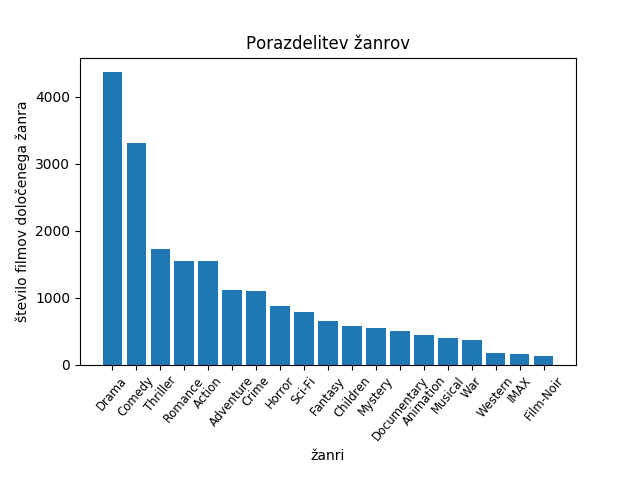
\includegraphics[scale=0.7]{slike/graph1_porazdelitev_zanrov.png}
			\caption{Prikaz žanrov in število njihovih pojavitev}
			\label{slika1}
		\end{center}
	\end{figure}
	Več o sliki si lahko preberete v razdelku Priloge - Slike.
	
	\section{Relacija med ocenami in gledanostjo}
	Pri tej nalogi sem moral ugotoviti relacijo med gledanostjo filma in povprečno oceno iz datoteke ratings.csv
	
	Koliko je film gledan v tej množici podatkov definira število ocen (bolj je film gledan, več ima ocen). Povprečno oceno filma sem pa lahko uporabil iz naloge 1 (Najbolj ocenjeni filmi).
	Za vsak film sem preštel kolikokrat je ocenjen in izračunal njegovo povprečno oceno:
	
	\begin{figure}[htbp]
		\begin{center}
			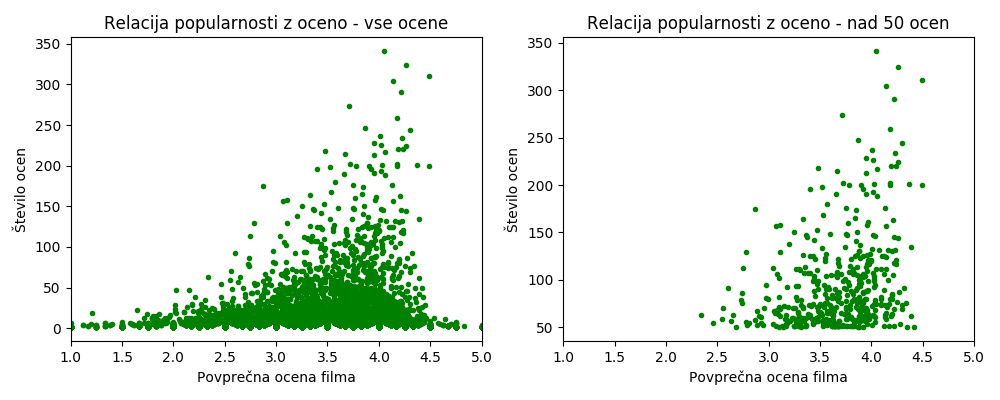
\includegraphics[scale=0.7]{slike/graph2_popularnost_ocena.png}
			\caption{Leva slika predstavlja število vseh ocen in njihovih povprečnih vrednosti, desna slika pa število filmov z vsaj 50 ocenami}
			\label{slika2}
		\end{center}
	\end{figure}

	Pri zgornji sliki se jasno vidi da število ocen naredi razliko: več kot je ocen, bolj se točke prikažejo na desni strani grafa (pri oceni 5), saj dobre filme ljudje več gledajo in zato bolj ocenjujejo.
	
	Več o sliki si lahko preberete v razdelku Priloge - Slike.
	\section{Spreminjanje popularnosti filmov}
	Pri tej nalogi sem moral ugotoviti relacijo med časom in oceno filma iz datotek ratings.csv in movies.csv
	
	Od določenega filma sem pridobil vse ocene in kdaj so bile te cene vpisane. Te ocene sem potem razdelil na določen interval in naredil povprečje iz tega.
	
	Pri večjih intervalih(50 in 100) se ni videl poseben trend, saj je premalo ocen da bi lahko te ocene združil v tako velike intervale. Tako da sem združeval v manjše intervale po 20 ali celo po 10
	
	Filmi ki so imeli premalo ocen je bilo nesmiselno združevati v intervale, zato sem te izpustil
	
	Ocene filmov skozi čas zelo nihajo. Najboljši primer tega je znan Pulp Fiction (1994) (na sliki spodaj levo)
	Zanimiv je tudi graf filma Schindler's List (1993), ki po dosežku ocene 5 začne ocena kar padati.

	\begin{figure}[htbp]
		\begin{center}
			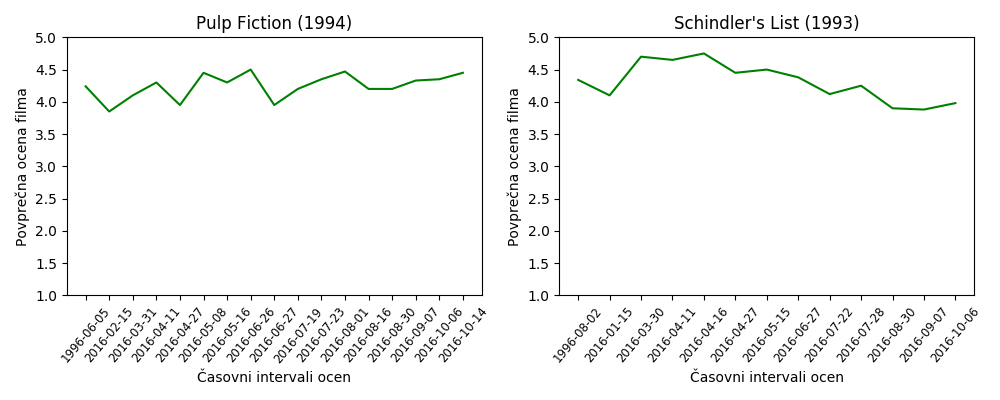
\includegraphics[scale=0.7]{slike/graph3_pulp_schindlers.png}
			\caption{Na levi sliki je film Pulp Fiction in njegove ocene na časovnih intervalih, na desni pa Schindler's List (vzorčenje po 20 ocen)}
			\label{slika3}
		\end{center}
	\end{figure}
	Več o sliki si lahko preberete v razdelku Priloge - Slike.
	
	
	\section{Popularnost igralcev}
	Popularni so tisti igralci, kateri imajo veliko pojavitev v filmih ki so dobro ocenjeni in velikokrat ocenjeni.
	Tako da potrebujemo vsoto nekega faktorja ki bo določal koliko je film popularen. Ta faktor sem dobil tako, da sem dobil procent, koliko ima film število ocen v primerjavi s številom ocen najbolj popularnega filma. To se pravi filmi z večjim procentom imajo več ocen. Ta procent sem potem pomnožil z oceno filma. Če imata dva filma isto število ocen bo zmagal tisti, ki je v povprečju bolje ocenjen.
	
	Formula zgleda nekako tako:
	
	\begin{lstlisting}
	for film in igralec.movies():
		utez = film.stevilo_ocen / maksimalno_stevilo_ocen
		igralec.popularnost += utez * film.povprecna_ocena
	
	\end{lstlisting}
	
	Najbolj popularni igralci pa so naslednji:\\
	\begin{lstlisting}
	Harrison Ford
	Tom Hanks
	Bruce Willis
	Robert De Niro
	Morgan Freeman
	Brad Pitt
	Kevin Spacey
	Tom Cruise
	Bill Murray
	Steve Buscemi
	\end{lstlisting}
	Prav tako sem opazil, da imajo filmi veliko manjkajočih vrednosti za avtorje. Tako da sem moral odstraniti te zapise.
	\section{(bonus) Najljubši film}
	Moj najljubši film je Inception (2010, Christopher Nolan), saj ima posebno idejo koliko so naši možgani zmožni in implementira dobre časovne trike.
	

	\section{Izjava o izdelavi domače naloge}
	Domačo nalogo in pripadajoče programe sem izdelal sam.
	
	\appendix
	\appendixpage
	\section{\label{app-res}Slike}
	Slike sem priložil v mapo slike.
	
	Slika1: graph1 porazdelitev zanrov:
		Na sliki je na x osi predstavljenih 19 žanrov, na njihovih y oseh pa število filmov, ki pripadajo temu žanru. Najbolj izstopata žanra "Drama" in "Comedy"
		
	Slika2: graph2 popularnost ocena:
		Na sliki sta 2 grafa, ki se pa razlikujeta o minimalnem številu ocen ki so prikazane.
		Oba grafa graf prikazujeta povprečne ocene filmov na osi x in koliko ocen ima ta film po oceni x, vendar levi graf nima spodnje meje pod koliko naj ocene ignoriramo.
		Ocene bi ignorirali zato, ker majhno število ocen pokvari graf, saj te niso pravilno uravnotežene. To tukaj lahko dobro vidimo, saj ima levi graf veliko večjo varianco kot desni, kjer so ocene že bolj stabilizirane.
		
	Slika3: graph3 pulp schindlers:
		Na sliki sta dva grafa, ki prikazujeta povprečno oceno filma in njihove časovne intervale za dva filma:
		Na levi sliki je predstavljen film Pulp Fiction (1994), kjer ocene zelo nihajo, vendar so v povprečju zelo na horizontalni črti. Na desnem grafu je pa film Schindler's List (1993), kjer pa tudi nihajo ocene, ampak začnejo po prvi četrtini leta 2016 ocene padati.
		
	
		
	\section{\label{app-code}Programska koda}
	Programsko kodo sem zapakiral v datoteko koda.zip in jo priložil k poročilu.
	Prav tako sem v ta zip priložil datoteke potrebne za zagon programa.
	Za zagon programa odprite main.py datoteko in v funckciji main odkomentirajte funkcijo ki jo hočete testirati.

	
\end{document}
